\documentclass[1p]{elsarticle}
\usepackage{amssymb, graphicx}
\usepackage{pbox}
\usepackage{natbib}
\usepackage{url}
%\usepackage{hyperref}
\begin{document}

\begin{frontmatter}



\title{Mantid - Data Analysis and Visualization Package for Neutron Scattering and $\mu SR$ Experiments}

% use optional labels to link authors explicitly to addresses:
% \author[label1,label2]{}
% \address[label1]{}
% \address[label2]{}
\author[tessellaUK]{O.~Arnold}
\author[ornl]{J.~C.~Bilheux}
\author[ornl]{J.~M.~Borreguero}
\author[isis]{A.~Buts}
\author[ornl]{S.~I.~Campbell}
\author[ill]{L.~Chapon}
\author[isis]{S.~J.~Cottrell}
\author[ornl]{M.~Doucet}
\author[tessellaUK]{N.~Draper}
\author[isis]{R.~Fowler}
\author[tessellaUK]{M.~A.~Gigg}
\author[ornl] {M.~E.~Hagen}
\author[isis]{A.~Hillier}
\author[ornl]{V.~E.~Lynch}
\author[isis]{P.~Manuel}
\author[isis]{A.~Markvardsen}
\author[isis]{R.~L.~McGreevy}
\author[uws,ornl]{D.~J.~Mikkelson}
\author[uws,ornl]{R.~L.~Mikkelson}
\author[nccsornl]{R.~Miller}
\author[isis]{K.~Palmen}
\author[isis]{P.~Parker}
\author[isis]{G.~Passos}
\author[isis]{T.~G.~Perring}
\author[ornl]{P.~F.~Peterson}
\author[isis]{F.~Pratt}
\author[ornl] {Th.~Profen}
\author[oxford]{P.~G.~Radielli}
\author[ornl]{S.~Ren}
\author[ornl]{M.~A.~Reuter}
\author[ornl]{A.~T.~Savici}
%\corref{cor1}\footnote{For general Mantid correspondence use %\texttt{mantid-help@mantidproject.org}}}
%\ead{saviciat@ornl.gov}
\author[isis]{J.~W.~Taylor}
\author[tessellaUS,ornl]{R.~J.~Taylor}
\author[tessellaUK]{R.~Tolchenov}
\author[isis]{R.~Whitley}
\author[ornl]{W.~Zhou}
\author[ornl]{J.~Zikovsky}

\address[ornl]{Neutron Data Analysis and Visualization, Oak Ridge National Laboratory, Oak~Ridge,~TN,~USA}
\address[tessellaUK]{Tessella Ltd., Abingdon, Oxfordshire, UK}
\address[isis]{ISIS Facility, Rutherford Appleton Laboratory, Chilton, Didcot, Oxfordshire, UK}
\address[ill]{Institut Laue-Langevin, Grenoble, France}
\address[uws]{University of Wisconsin-Stout, Menomonie, WI, USA}
\address[nccsornl]{Computing and Computational Science Directorate, Oak Ridge National Laboratory, Oak~Ridge,~TN,~USA}
\address[tessellaUS]{Tessella Inc., Newton, MA, USA}
\address[oxford]{Department of Physics, University of Oxford, New Parks Road Oxford, UK}



\begin{abstract}
The Mantid framework is a software solution developed for analysis and visualization of neutron scattering and muon spin measurements. The framework is jointly developed by a large team of software engineers and scientists at the ISIS Neutron and Muon Facility and the Oak Ridge National Laboratory.  The objective of the development is to improve software quality, both in terms of performance and ease of use for the the user community of large scale facilities. 
The functionality and novel design aspects of the framework are described.
\end{abstract}

\begin{keyword}
% keywords here, in the form: keyword \sep keyword
Data analysis \sep Data visualization \sep Computer interfaces
% PACS codes here, in the form: \PACS code \sep code
\PACS 07.05.Kf 	%Data analysis: algorithms and implementation; data management (for data analysis in nuclear physics, see 29.85.-c)
\sep 07.05.Rm 	%Data presentation and visualization: algorithms and implementation 
\sep 07.05.Wr 	%Computer interfaces (for nuclear physics applications, see 29.50.+v)
\end{keyword}
\end{frontmatter}

% main text
\section{Introduction}
\label{Introduction}


The use of large scale facilities by researchers in the field of condensed matter, soft matter and the life sciences is becoming ever more prevalent in the modern research landscape. Facilities such as Spallation Neutron Source (SNS) and High Flux Isotope Reactor (HFIR) at Oak Ridge National Laboratory (ORNL) and ISIS at Rutherford Appleton Laboratory (RAL) have ever increasing user demand and produce ever increasing volumes of data. One of the single most important barriers between experiment and publication is the complex and time consuming effort that individual researchers apply to data reduction and analysis.

The objective of the Manipulation and Analysis Toolkit for Instrument Data or Mantid framework is to bridge this gap with a common interface for data reduction and analysis that is seamless between the user experience at the time of the experiment and at their home institute when performing the final analysis and fitting of data.

The Mantid project is a large international collaboration between the Science and Technology Facilities Council (STFC) (UK) and the Department of Energy (DOE) (US) to co-develop a high performance computing framework for analysis of: powder and single crystal neutron diffraction data, inelastic and quasi-elastic neutron scattering data, polarised neutron diffraction data, neutron reflectometry data, small angle neutron scattering data and $\mu SR$ data. 

The Mantid framework consists of a highly modular C++/Python architecture which supports user built plug-in functions as well as access to powerful visualization toolkits such as ParaView\cite{paraview}. This modular design allows users to easily extend the capability of the framework to almost any application. The framework is provided under the GNU General Public Licence version 3\cite{gpl}, and is built for all commonly used operating systems.


In the past, each instrument (or instruments groups at a given facility) would develop individual bespoke software routines for their own science areas\cite{DAVE, OpenGenie, LAMP, ISAW}, over the life of a facility $>$40 years this leads to a vast unmanageable library of mission critical software routines. Such a model is prone to single point failures as individual authors of software leave a facility they take with them the key knowledge of the software they developed. This often leads to refactoring of existing code as the facility attempts to get back control of its mission critical software. 

In this article we describe the Mantid framework and its novel features. Mantid has been developed with the overall objective of giving facilities and their users access to state of the art bespoke software that is professionally developed and maintained, with a clear science led strategic development and maintenance plan.
%The manner in which the Mantid framework has been developed is a paradigm shift in software development at large scale facilities. The previous single developer model has been superseded at ISIS and SNS by a well resourced development team. 
This methodology allows instrument scientists time to determine key software requirements for their user programmes rather than having to develop and maintain software packages, in so doing both the user community and the facility benefit.

The overall ethos of the project is that of abstraction. That is to say, code developed within the project should at all times operate on all data types from all participating facilities. This idea leads to a framework that is, in principle, easier to use and maintain.

The Mantid project\cite{mantiddoi} was started in 2007 at ISIS, and joined by SNS and HFIR in 2010, with the goal of implementing a new framework for data analysis and visualization for neutron scattering and $\mu SR$ experiments. 
The main objectives for the project are:
\begin{itemize}
\item To provide a technique independent, neutron and muon specific framework  to reduce, visualise and perform scientific analysis of data
\item To ensure quality by following professional software development practices
%\item Core framework aspects are developed using change control project management practices 
\item To actively support multiple platforms (Linux, OS X, Windows)
\item The software, source and documentation will be freely distributable
\item The framework must be easily extensible by instrument scientists and users
%\item The framework must provide both low level functionality for advanced uses, and high level, and high level, simple and intuitive interfaces for standard measurements 
\item Provision of comprehensive, well maintained documentation
\end{itemize}

\section{Neutron scattering}

Neutron scattering is an established technique for determining the structure and dynamics of materials. It has generated a large user community with research interests from life sciences to quantum magnetism. To meet the current and future demands in these areas, there have been a number of new large scale facilities built, or in the process of being built in the last 10 years. These new facilities are all pulsed spallation neutron sources rather than reactors. Pulsed spallation sources by definition have a time structure to the neutron production and, as a result of this, all instruments operate in a detection mode known as time of flight (TOF). TOF neutron instruments have the advantage of being able to collect data over a wide range in $S(q,\omega)$ in a single pulse. 
In a neutron experiment one must relate measured counts to the physically meaningful $S(q,\omega)$.

At a modern TOF neutron source it is common for instruments to have $10^5 n\ cm^{-1}s^{-1}$ and millions of pixels, generating GB size data files. In many experiments it is possible for several files to be combined together to create a large $n$ dimensional dataset or volume with a size of up to 1 TB.
Recently pulsed sources have started to collect data in what is called event mode. This method simply lists to a file every detected neutron with a time of collection and other metadata. From the event list, one may filter based on time or metadata to create data subsets. This method has several advantages, it is effective for storing sparse data, it allows time resolved experiments to be performed. 
Large data volumes, $n$ dimensional data and event mode format add several layers of complexity to the data reduction chain. For the instruments to be fully exploited, high performance software is a necessity. 



\section{Muon Spin Relaxation/Rotation/Resonance ($\mu SR$) }

Muons provide a local probe to investigate the properties of a wide range of materials. 
$\mu SR$ has wide applicability and provides useful dynamic information for a broad range of science  from soft matter to quantum magnetism,  which is often complementary  to that from neutron scattering. 
The technique is similar to that of nuclear magnetic resonance, in which the polarisation of the target nuclei, in this case the muon, is tracked as a function of time. 
In the case of muons, spin polarised muons are implanted into the material under investigation and these muons decay into  positrons which are emitted preferentially along the final spin direction of the muon. 
By time stamping the detected positrons the muon polarisation is inferred. As muons are produced by the decay product of pions, which in turn are produced by high energy protons ($\sim$800 MeV at ISIS), experiments are conducted at proton accelerators and are often situated next to spallation neutron sources, e.g. ISIS, PSI and J-PARC. 
This means that the users of neutron instruments often use muons as well and having a familiar software framework for analysis is clearly beneficial.
The Mantid framework fulfils this requirement, comprising  a wide range of methods with which to analysis the muon depolarisation spectrum:  integrated asymmetry, Fourier transform, maximum entropy and time domain analysis among others. 
Moreover, simulations of muon data using Density Functional Theory or electronic calculations can yield further insights into the material under investigation. 
The ability to link these simulations with the data analysis with a simple interface yields a very powerful tool for the analysis of muon experiments. Again, the Mantid framework offers this functionality to the instrument user.



\section{Development Practices}
One of the key  aspects of Mantid is the manner in which it is developed. 
In order to achieve the stated goals, a large team of scientists and scientific software engineers in Europe and United States are collaborating on this project. For an effective collaboration, we use several software development tools and practices designed to support distributed development teams. New feature requests or defect reports are entered into an issue tracking system. %Mantid  uses  \textit{Trac} \cite{trac} for this purpose.
 
Another tool vital for organising work is the use of a version control system. Mantid uses git \cite{git} repositories% hosted at GitHub \cite{github}
 for the source code, configuration files, and much of the documentation. To allow multiple developers to work in similar areas without interference, developers work on separate branches for each feature. To verify that there are no cross-platform compatibility issues, each feature branch is merged onto a 'develop' branch whenever new code is ready. It is only after a feature branch has been completely addressed and tested that the code changes are merged onto the 'master' branch from which release builds and new features are based.

In order to ensure quality, the Mantid project uses continuous integration.
% built around the Jenkins continuous integration server\cite{jenkins}. 
Whenever new code is committed to the 'develop' branch, builds for each supported operating system are started, and are tested against a suite of over 6000 automated unit tests. A build is marked successful only if all of these unit tests pass. 
%Every night, a nightly build of the 'master' branch is done once a day. 
Once a day, a series of over 150 integration 'system tests' are run with the most recent locally installed version. Builds that pass all system tests are immediately available for download and, in some cases, automatically deployed to computers. Formal releases of Mantid occur approximately every three months, and undergo additional manual testing. These releases are accompanied by detailed release notes and training. 


\section{Mantid Design}



One of the main design consideration for this project was the separation of data and algorithms. The ethos of the development is that algorithms should (where possible) operate on all data types without \textit{a\ priori} knowledge of the data or the experiment that generated it. In principle, this ideology makes the framework cleaner and easier to use. In many instances, scientists are not experts in neutron scattering, $\mu$SR, or the associated data analysis that is required. Successful software application written for scientists must take this into account at the design stage.

Data containers (called workspaces) and algorithms, which manipulate workspaces, compose the central element of the Mantid Framework (Figure \ref{fig:Framework}). 
Workspaces and algorithms are aware of the geometry of each individual instrument. 
%Instrument geometries are XML files containing the real space position of all instrument components.
\begin{figure}[!ht]
\centerline{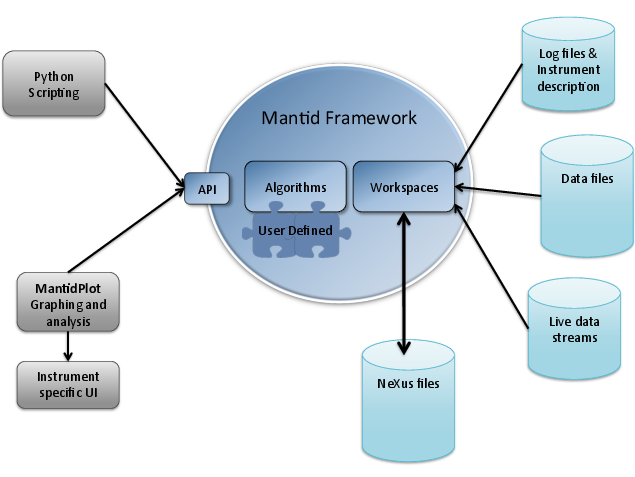
\includegraphics[width=0.75\textwidth]{MantidFramework.png}}
\caption{Mantid Framework design}
\label{fig:Framework}
\end{figure}
Workspaces can be loaded from various file formats, live data streams, or created by different algorithms. The workspaces can be manipulated by the many algorithms in Mantid, and saved in a variety of formats. By default, Mantid uses the NeXus format\cite{NeXus} for saving intermediate and processed data, but various other output formats are also supported.

To ensure high performance for data analysis, but also allow flexibility in how the data is processed, the project is written in C++ with Python bindings. For parallel processing, Mantid uses OpenMP\cite{openmp}, Posix threads and MPI\cite{mpi}. The interaction with the Mantid Framework occurs through the application programming interface (API). Currently the main interactions occur through either Python or through the graphical interface. 

%The key features of the framework are:
%\begin{itemize}
%\item Powerful data container workspaces handling multiple data types, experiment logs and experiment metadata
%\item Abstracted algorithms
%\item Inbuilt instrument geometry and solid geometry handling 
%\item Handling of multiple data types including event mode data
%\item Python bindings for all aspects of the core framework 
%\item Platform independent code
%\item Multiple platform builds along with platform specific installers for Mantid, Python, IPython, SciPy and NumPy
%\item The framework is OpenMP aware and designed to maximise performance on multicore machines
%\end{itemize}

\subsection{Instrument Geometry}
A full description of the instrument is used within the Mantid framework. One way to specify the geometry is the instrument definition file (IDF). The IDF is a XML description of all pertinent instrument components.% (Table \ref{IDF}). 
The IDF component description can be expanded upon to increase the information level accessible to the Mantid framework. 
Previous applications for neutron scattering data analysis have generally only described instruments by their primary and secondary flight paths and detector angles. A full description, based on constructive solid geometry, allows complex visualization of the instrument and its detectors, along with the possibility to perform Monte Carlo simulations.
To account for moving instrument components, the instrument geometry is updated using log values. %The solid geometry engine within the Mantid framework can be used to described complex sample shapes to allow absorption correction to be made.

%\begin{table}[htdp]
%
%\footnotesize
%\begin{tabular}{l | c | c }
%Component type & Position information &Supplemental information \\ \hline
%Beam Monitor& flightpath position& Monitor type Gas / scint\\
%Detector&X,Y,Z r,$\theta$,$\phi$& detector type gas/scint gas pressure wall thickness\\
%Neutron guide&dimensions /length &m factor\\
%Beam Chopper&slit dimensions&speed\\
%Beam defining slits&dimension\\
%Source type&dimension &type /temperature
%
%
%\end{tabular}
%
%\caption{Component types currently stored in the instrument definition in Mantid together with possible position information and metadata}
%\label{IDF}
%\end{table}%

%\subsection{Classes}
%\textbf{is this required too}

\subsection{Data Types}
The Mantid framework is capable of reading a variety of data types. The most commonly used are data files written in the nexus standard. However the framework can read legacy files from ISIS as well as generic x,y,e ascii data. Generic and histogram data and read info the workspace2D type of data container. instrument data are populated alongside the IDF description of the instrument. Event mode nexus files are read into event workspaces and can be filtered on $TOF$ at load. 
Alongside the standard loading of a pre-existing datafile Mantid can also access the instrument data directly to provide real time display of detector counts and live 'on the fly' data reduction. 

\subsection{Workspaces}
Workspaces are the data containers in Mantid. In addition to the data, workspaces can hold other types of information, such as instrument geometry, lattice parameters and orientation, or sample environment logs. Each workspace also holds its history, a list of algorithms that were used to create that workspace. That way each workspace can prove it's provenance, and also regenerate the commands used to make it. Depending on the organization of the data, there are various types and subtypes of workspaces. Table \ref{workspaceTable}


\begin{table}[htdp]

\footnotesize
\begin{tabular}{ p{0.16\textwidth} |  p{0.12\textwidth} |  p{0.2\textwidth}|   p{0.2\textwidth} |  p{0.12\textwidth}}
Workspace type & Data format & Mode &Metadata&Uses\\ \hline
&&&&\\

Workspace2D	& X,Signal, Error & Histogram / point& sample logs, Spectrum Number, detectorID&raw data\\
&&&&\\

EventWorkpsace&eventlist	&on the fly rebin   correlated sample log, spectrum number, detector ID&raw event data	\\
&&&&\\
MDWorkspace & $n$ eventlist, $n$ histogram& adaptive mesh rebin& $n$dim, axis, units, sample logs& processed volume data sets\\
&&&&\\
TableWorkspace&column - row format& | &|& fitting results\\
\end{tabular}

\caption{Workspace types in Mantid together with type of data stored, metadata and current uses in the framework for each type of workspace}
\label{workspaceTable}
\end{table}%

Workspace2Ds contain data for multiple spectra, in the X, Signal, Error format, where X is a coordinate such as time of flight or energy transfer. 

The data acquisition system at several facilities now allow separate recording of each  detected neutron, and labelling it with time-of-flight, and wall-clock-time stamps. For each spectrum, the EventWorkspace contains a list of events \cite{EventPaper}. 

EventWorkspaces can also provide a histogram representation as well,which is calculated on the fly when requested. This allows event workspaces to support the MatrixWorkspace interface, also being supported by Workspace2Ds. The result is that algorithms and plotting work on the two types of workspaces interchangeably, without the need to know the details of how their data is stored. 
There are various uses for event workspaces. One can filter out unwanted events, such as events recorded during temperature spikes. The other big use for events is allowing novel techniques, such as asynchronous parameter scans (continuous angle scans, temperature scans), and pump probe experiments (pulse magnets, high frequency deformations of materials, and so on).

For data formats that contain different field types, Mantid provides various TableWorkspaces. A table workspace is organised in columns. Each column has a name and a type - the type of the data in that column. Examples of table workspaces are the model parameters from model fitting, and PeaksWorkspaces, a representation of information about Bragg peaks, that is used in crystallography experiments.
 
The last major workspace type is the multi-dimensional workspace, or MDWorkspace. While for matrix workspace there are two dimensions describing a data point (spectrum number and X coordinate), for MDWorkspaces we have between 1 and 9 dimensions. Higher number of dimensions are required to accommodate labelling of data with extended parameter dependencies, $i.e.$ sample environment variables. 
MDEventWorkspaces are adaptively rebined onto a mesh that is dependent on the number density of events Fig\ref{mdevent}.

\begin{figure}[!ht]
\centerline{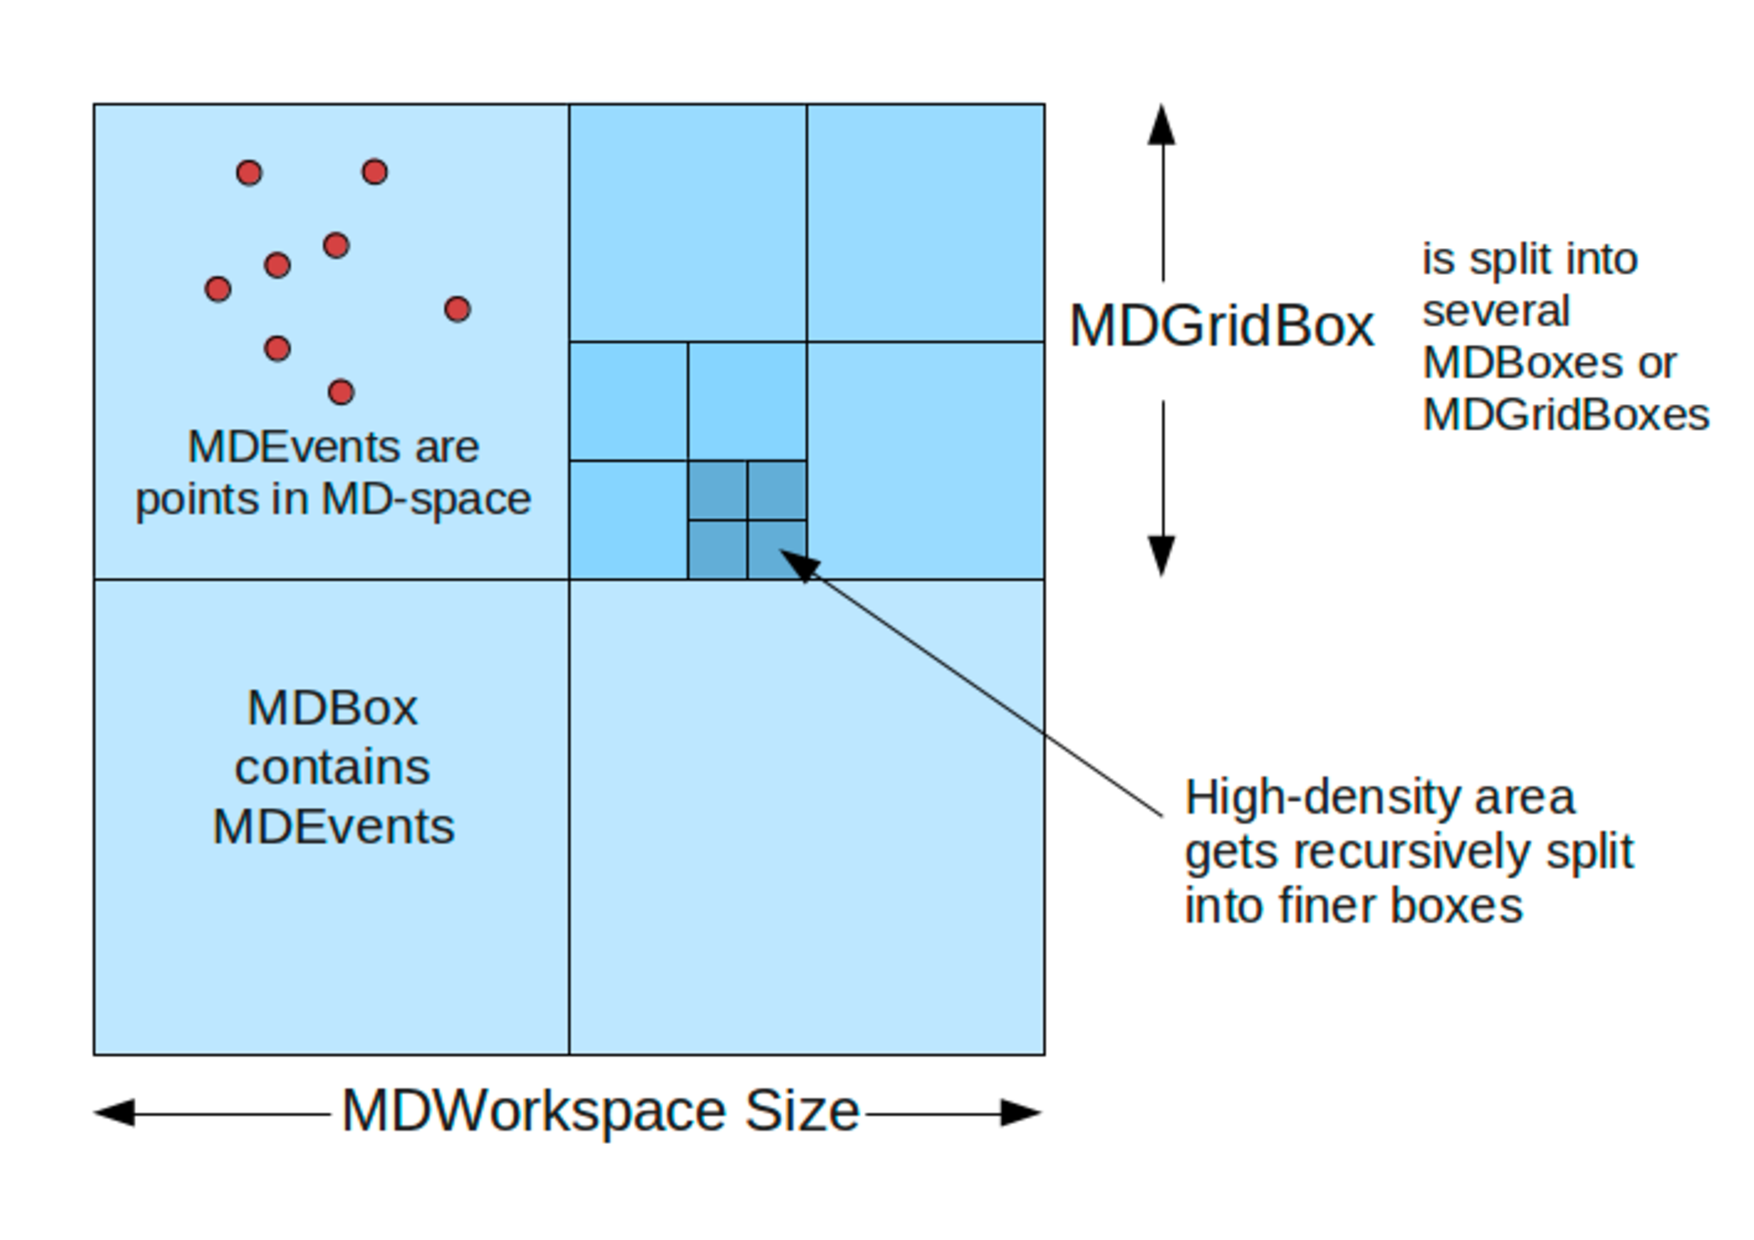
\includegraphics[width=0.75\textwidth]{mdevents.pdf}}
\caption{Schematic representation of the principle of adaptive rebinning used in the MdEventWorkspace type.}
\label{mdevent}
\end{figure}

For MDEventWorkspaces, each MDEvent contains coordinates, a weight and an error. It might contain also information about which detector and which run it comes from. All MDEvents are contained in MDBoxes. Above a certain threshold, the MDBox becomes an MDGridBox, by splitting into several equal size MDBoxes. This allows for an efficient searching and binning, and allows plotting on an adaptive mesh. 
MDHistoWorkspaces consist of signal and error arrays on a regular grid.  

\subsection{Algorithms}
Mantid algorithms are procedures to manipulate workspaces. They can be predefined, or written by users, in either C++ or Python. The algorithm layer is a key aspect of the Mantid framework. The organisation and development of algorithms is key to maintaining the ethos of the project; that is all algorithms should operate on all data for all instruments. This ethos therefore presents a number of challenges for development. The framework can access multiple data types, including event mode data. As a result of this the algorithm layer must be able to cope with multiple data type input and at the same time maximise performance for individual data types. The case of event mode data in interesting as it presents an efficient way of processing sparse data. It is often more efficient to keep the data as events through a chain of operations. This requirement has resulted in development of a number of event specific data handling operations. The end result is that for many reduction chains the data is event type until the final rebin for presentation. The key advantage of this for the end user is flexibility.

Core algorithms can be grouped together to form bespoke data reduction and analysis for individual instruments and science areas. These large algorithms can then be presented to the user at the python scripting layer, command line interface or as a custom reduction user interface. 

At the present, there are over 500 algorithms covering data handling (loading/saving workspaces from/to files), arithmetic operations(plus, minus, multiply), unit conversions, and many technique specific algorithms (powder diffraction, single crystal diffraction, SANS, reflectometry, direct and indirect spectrometry, and $\mu SR$).  

%%A particularly important set of algorithms was designed to deal with event data formats, to allow filtering and binning.

%%Algorithms can also be used to perform part of the work within other algorithms. This is particularly used within workflow algorithms, that specify a predefined series of steps to analyse particular data types within Mantid, starting with the raw files from the data acquisition system, and all intermediate stages, up to a format that scientists can work with.

%%Simple formatting, and input validation can transform user scripts in algorithms, and these can be shared with the entire Mantid community using the Mantid Script Repository, or by submitting them to the development team, to be included in the installation packages


\subsection{Python API and scripting}
The python API for the Mantid framework provides an exceptionally powerful interface to the core C++ framework. All classes within the framework are open to python control, with the algorithms be added to the API at run time, allowing new plug in algorithms to be available without further configuration. The python API can be used to simply interact with algorithms and workspaces or as a method to quickly expand the framework with new functionality. 

The API has been written to give a intuitive command line interface feel, allowing simple powerful syntax with a minimal understanding of the Python language.  More advanced usage is possible within python scripts allowing popular packages such as numpy or scipy to be mixed with Mantid Algorithms to process data.  Furthermore Python can also be used to extend the capabilities of the Mantid framework adding further algorithms or fit functions without needing to recompile or even restart the program.


%%The most flexible way to interact with the Mantid framework is through the python interface. By including the appropriate Mantid libraries, users can write their own reduction/analysis scripts, to execute their own custom reduction workflow. All algorithms implemented in C++ are automatically exposed to python. In addition, several methods related to workspaces, and other helper objects are available as well. A tutorial of using the Python API can be found in the Documentation section on the Mantid webpage\cite{webpage}.  

%%Most reduction procedures for a particular instrument follow the same pattern, with minor parameter changes to account for experimental conditions. If there is enough metadata in the input files to get the required parameters, the Python interface allows the reduction process to occur automatically, as soon as the raw data file is saved. This is the case for several instruments at SNS. 









\section{User Interface}
\subsection{MantidPlot}
The main interaction with Mantid occurs through the MantidPlot interface (Figure \ref{fig:MantidPlot}). It is a graphical user interface based on QtiPlot\cite{qtiplot}. It allows 1D, and 2D plots of the data, and access to the VATES interface for MDWorkspaces (see section \ref{VATES}). From the MantidPlot window, accessing the Python interface can be achieved through the script window (used to run entire scripts at once)  the script interpreter or python shell.

A searchable list of all algorithms is also present by default, organized in categories. Clicking on an algorithm will open an automatically generated dialog box, with entries for each of the input parameters. A quick validation occurs when information is filled, and if any input is invalid it is flagged with a error message for the user. For each algorithm dialog box, a button allows for invoking the built-in help. A results log window is also available, where users can see the results of running different algorithms. For several scientific techniques, custom interfaces are available from the MantidPlot menu.

\begin{figure}[!ht]
\centerline{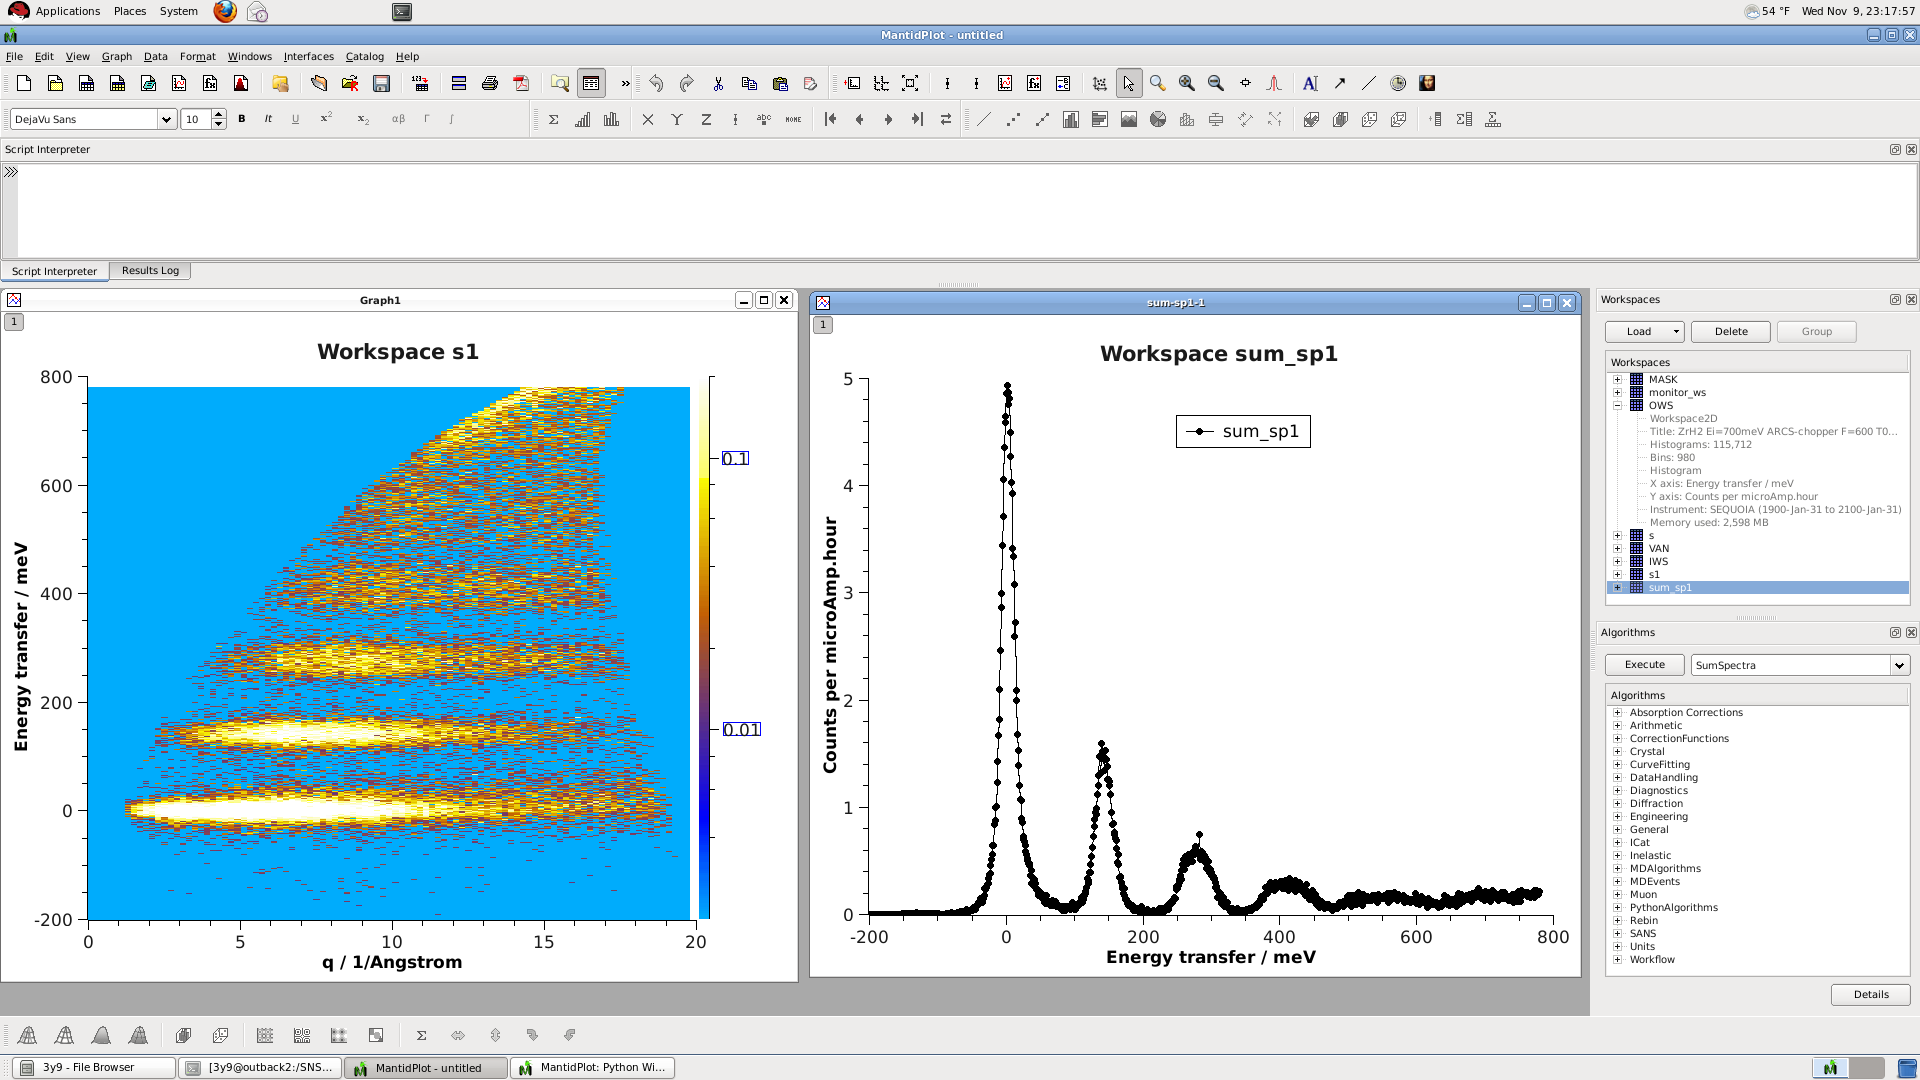
\includegraphics[width=0.75\textwidth]{MantidPlot.png}}
\caption{MantidPlot interface, showing 1D, and 2D plots. Lists of workspaces and algorithms are available on the right side}
\label{fig:MantidPlot}
\end{figure}
The Workspaces toolbox show a list of all the workspaces currently available, which may be hosted in the computer memory or on disk. Clicking on the workspaces show information about workspace type and content. A context sensitive menu allows simple plotting, instrument view, inspection of the sample environment logs, or a listing of the history of the workspace. 


\subsection{Data reduction and bespoke interfaces}
\begin{figure}[!ht]
\centerline{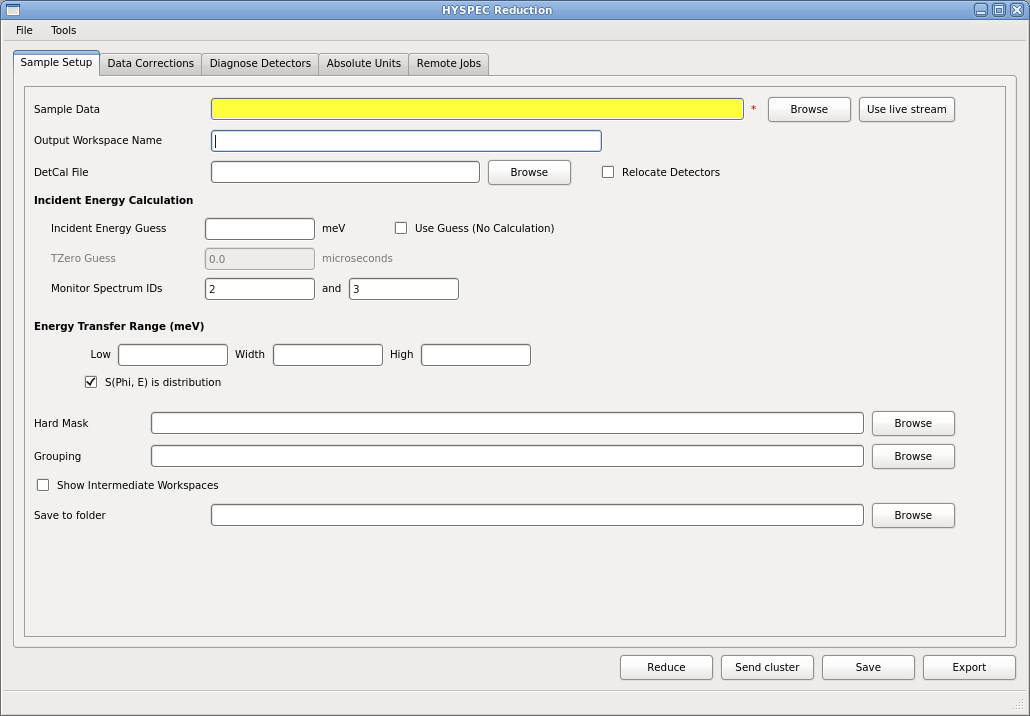
\includegraphics[width=0.75\textwidth]{Hyspec.png}}
\caption{Custom interface for direct geometry reduction on HYSPEC instrument}
\label{fig:Hyspec}
\end{figure}

Data reduction and basic analysis for individual instruments or science areas is generally a sequential chain of operations starting from data loading and resulting in a dataset that has physically intractable units. As such reduction scripts for several scientific techniques can be complicated, and depending on a large number of parameters. More often than not development of new features in this area must take into account legacy usage requirements and be well validated against existing "known" good results. In all cases development of data reduction chains are tightly controlled and validated. 

One of the objectives of Mantid is to provide the facility user with a simple and efficient interface to allow them to analyse their data.  To achieve this for multiple science areas and instruments a number of custom interfaces have been implemented to process data from specific experiments. 
These are presented to the user through a GUI layer and often a "workflow algorithm" 
A number of bespoke GUIs have been implemented to deal with utility functions useful for neutron science.
Science areas and instruments specifically supported by the Mantid framework can be seen in Table\ref{coverage}



\begin{table}[!htdp]

\footnotesize
\begin{tabular}{p{0.4\textwidth} |  p{0.4\textwidth} }
Science area &Instruments \\ \hline
Powder neutron diffraction&GEM HRPD WISH POLARIS POWGEN \\
Single crystal neutron diffraction&WISH SXD TOPAZ\\
Inelastic neutron scattering (direct)&MERLIN MAPS MARI LET SEQUOIA ARCS HYSPEC CNCS IN4 IN5 IN6 \\
Inelastic neutron scattering (indirect)&BASIS IRIS OSIRIS TOSCA VISION\\
Small angle neutron scattering &SANS2D LOQ EQ-SANS GP-SANS BIO-SANS D33\\
Neutron reflectometery&CRISP SURF POLREF INTER OFFSPEC \\
$\mu SR$&MUSR HIFI EMU\\
\end{tabular}
\caption{Current science areas and instruments supported by the Mantid framework}
\label{coverage}
\end{table}%

In some cases a single "workflow algorithm" is beneficial, one such case is for live event process. The application can access the live data steams of event mode instruments at SNS and ISIS and can directly read histogram data from the detector electronics of ISIS instruments. Fig \ref{live events} shows the generic workflow to process and view data as it is collected.
\begin{figure}[!ht]
\centerline{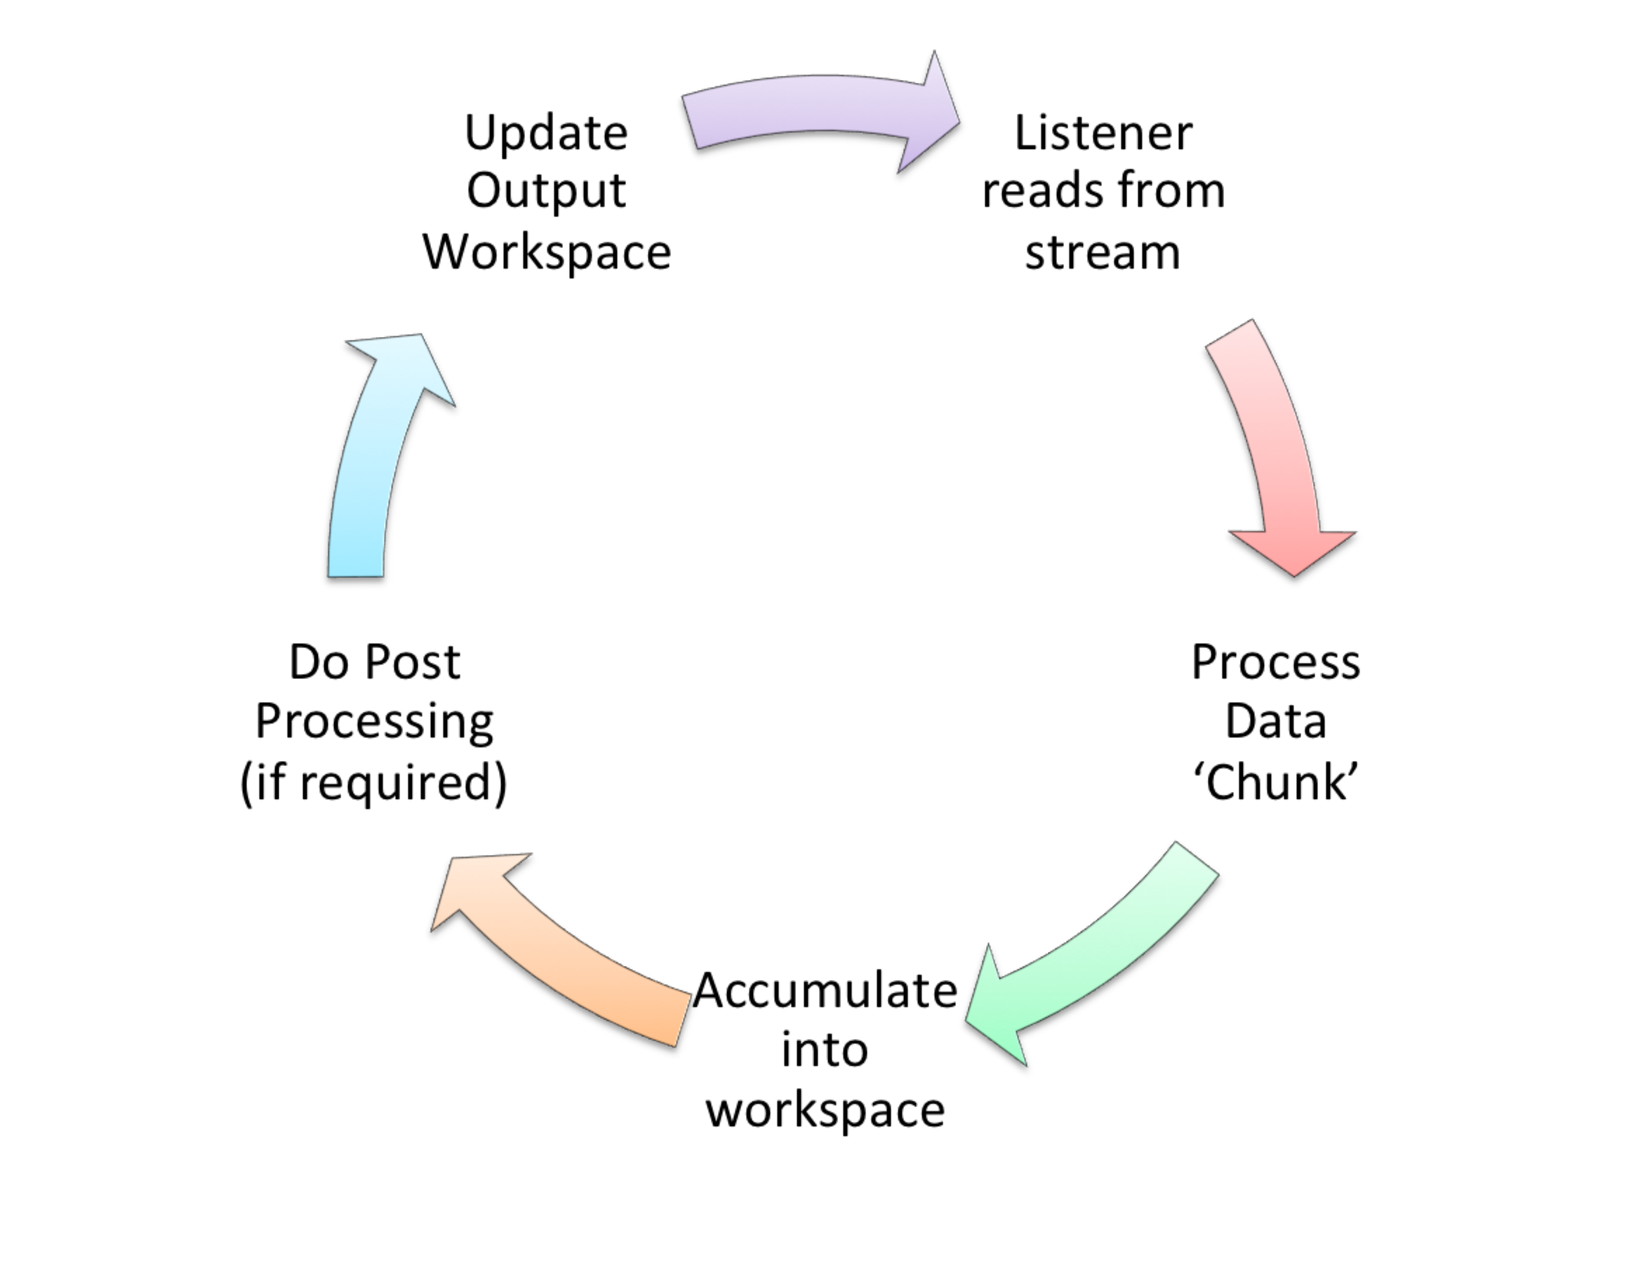
\includegraphics[width=0.75\textwidth]{liveevents.pdf}}
\caption{Flow diagram representing data flow when using live data processing within Mantid}
\label{live events}
\end{figure}




%%One can use either scripts of workflow algorithms to manipulate the raw data. The complexity of scripts can be intimidating for new users, while auto-generated dialog boxes for workflow algorithms can be unintuitive as well. Where needed, the development team, and sometimes individual instrument scientist, have created custom user interfaces, to make complex analysis workflows much easier to use.

The custom user interfaces, available from MantidPlot, group together inputs from related reduction parameters, and spread independent steps onto different tabs. Figure \ref{fig:Hyspec}, shows an example, the DGS Reduction interface for the HYSPEC instrument at SNS this is a generic reduction chain for inelastic neutron scattering instruments. 
%%When it is executed on computers with certain privileges, advanced option can appear or disappear, like live data analysis, or sending reduction jobs to particular computing clusters.

\textbf{Paz may need to expand on this}
The framework has inbuilt methods to process single crystal diffraction data, along with python routines to calculate  and refine the orientation matrix, index reflections integrate reflections and generate goniometer translations for crystal alignment.

\textbf{should we add more in this section about other types of reduction key features etc}

\subsection {Fitting}
Fitting mathematical functions and models to experimental data is a key requirement of any scientific computing application.
 The Mantid framework has implemented a powerful fitting engine for fitting multidimensional datasets.
 Fitting peak functions and simple user derived functions to line data i.e. data that is in 1D x,y,e format can be also performed using simple user friendly interface. This user interface has been developed to allow complex function to be created from simple mathematical building blocks using GUI. Any function or dataset can also be fitted within the scripting python interface.

Once the user has generated a model the subsequent fitting can be batch processed across many different datasets, with the option of plotting fit results against a log parameter. Output from the fit procedure is displayed as a Table Workspace dataset which can then be further manipulated and analysed to estimate statistical characteristics of fitting.


Figure \ref{fitting} shows the GUI used for fitting mathematical functions to 1D data.

\begin{figure}[!ht]
\centerline{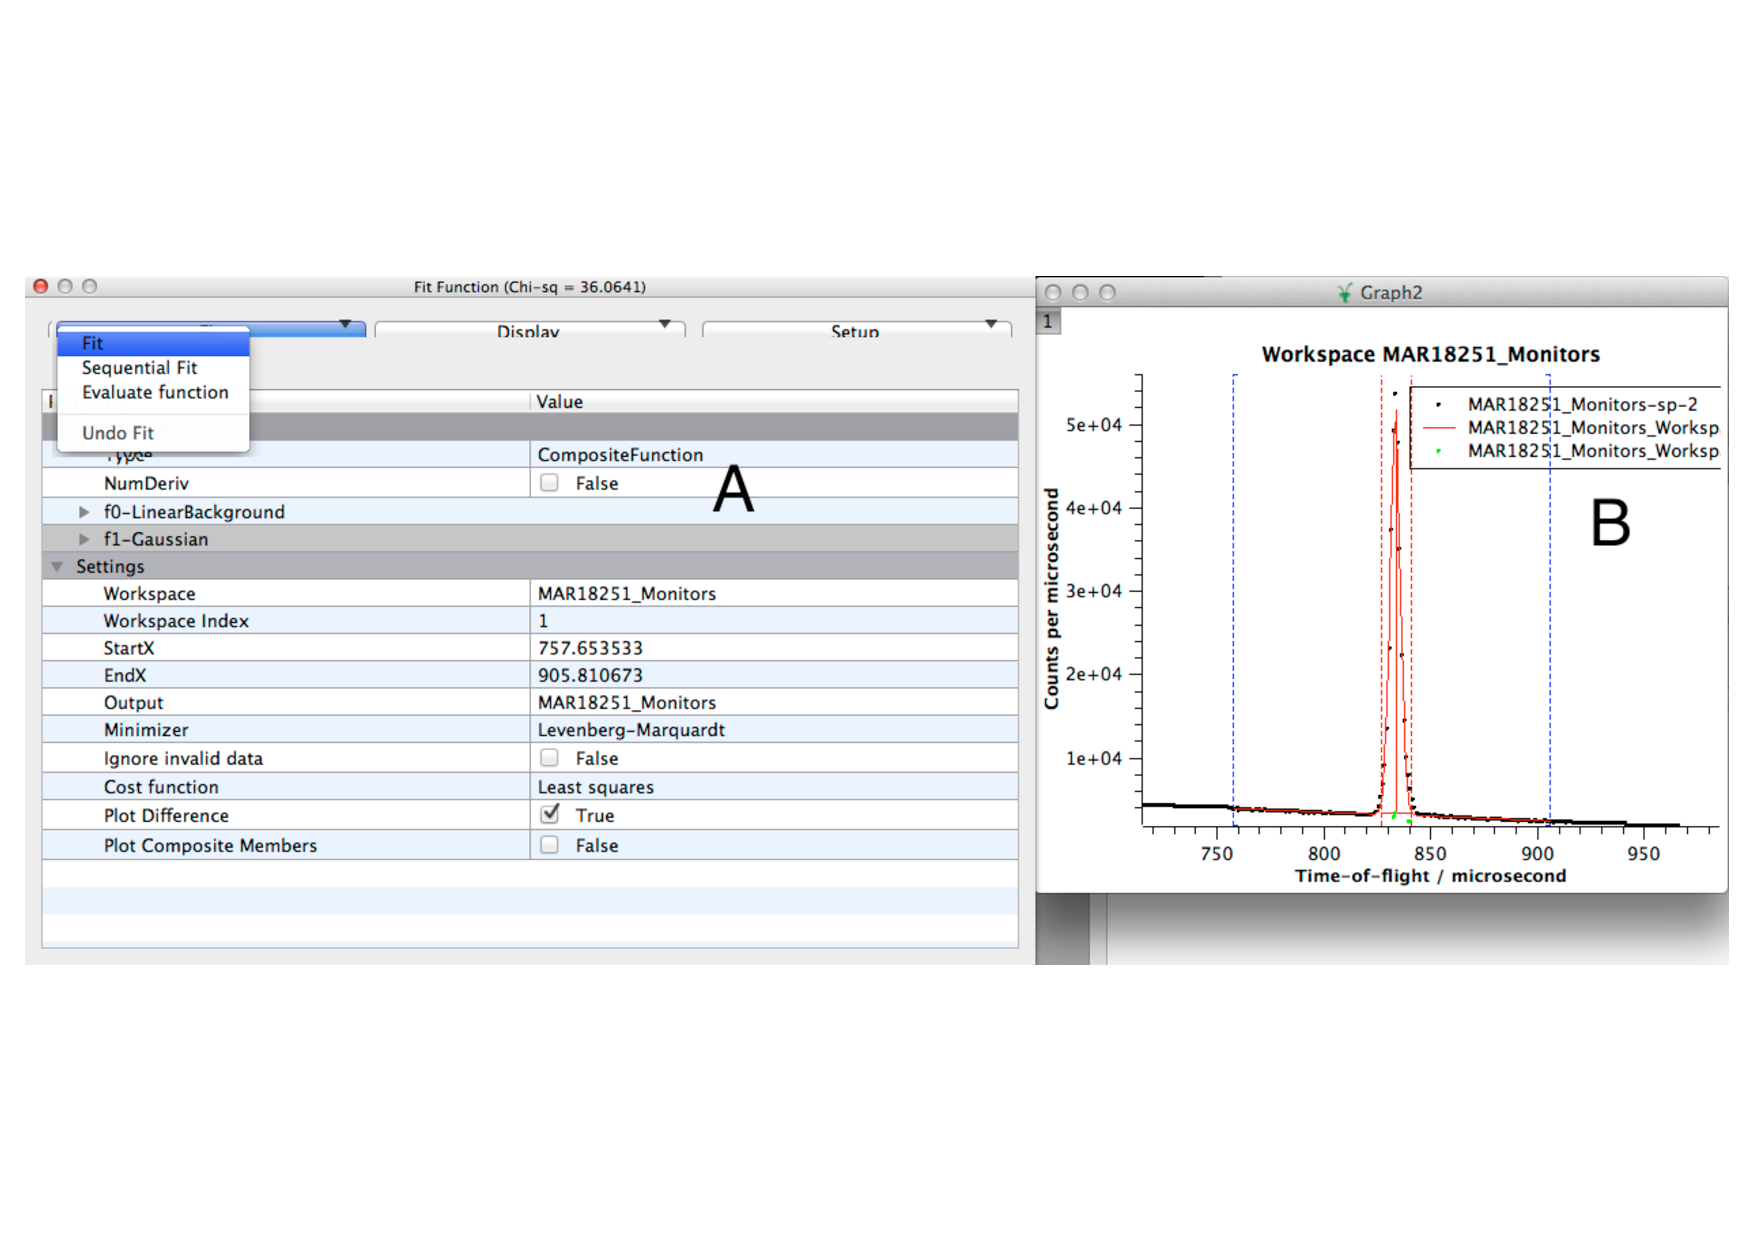
\includegraphics[width=0.75\textwidth]{fitting.pdf}}
\caption{The simple fitting GUI interface in the MantidPlot application. Peak selection is performed using mouse selection on the displayed data.
Panel A displays the required model and fit controls panel B displays the data, fitted model and difference the vertical dotted lines indicate extents in x for the model.  }
\label{fitting}
\end{figure}

There are a number of scientific techniques that always  fit complex function to reduced datasets in order to extract meaningful physical parameters. For the case of MUSR and QENS the Mantid framework fitting module is sufficient. For SANS the data can be output to external model fitting packages for further analysis. Mantid currently can link directly to $SASView$ for further analysis of experimental data.


\subsection {Simulation and Analysis}

Fitting over multidimensional datasets is used in more complex situations e.g. in the analysis of the results of the inelastic scattering experiments. Fitting a single resolution broadened model of scattering $S(q,\omega)$ to a $n$ dimensional $S(q,\omega)$ dataset is a standard data analysis procedure in this area used to account for substantial changes in the results of the experiment due to the instrument resolution effects.
 Mantid contains a set of procedures for calculating an instrument resolution function and convoluting this resolution with chosen scattering model to obtain simulated resolution broadened scattering model. It then can use the multidimensional fitting framework to compare simulated model scattering with experimental scattering and fit the parameters of the scattering model to the results of the experiments. These capabilities are similar to the capabilities available in the past program like $Toby$fit \cite{tobyfit}.At the moment $Toby$fit's Monte-carlo-based instrument resolution model is implemented in the Mantid and the framework allows to define and deploy other instrument resolution models. Mantid also already contains range of $Toby$fit's scattering models used in the analysis of the inelastic neutron scattering data.
 


\section{Visualization}

Modern multi detector instruments generate large data sets which cannot be easily visualised on a 1D graph or a 2D projection. 
Large position sensitive detector backs allow diffractometers and spectrometers to survey large areas of reciprocal space in a single experiment. 
A large multi detector instrument typically has 60-100k pixels visualising experimental data in real space of the entire instrument is often useful. For single crystal samples such instruments become large Laue geometry cameras. For SANS experiments area detectors of 1x1m are commonplace and place another requirement on visualization. 
For visualising the instrument data in real space the InstrumentView can be used (figure \ref{fig:InstrumentView}), and is described later. 

 
Often experiment perform crystal rotations to generate even grater maps of reciprocal space and for the case of inelastic neutron scattering that resolves both reciprocal space and energy transfer the data volume that is produced is in greater than 3 dimensions. 

Volumes of data are inherently large in memory and require special techniques to visualise  efficiently. Volume data in Mantid is encapsulated in the MDevent workspace type which uses dynamic box rebining to maximise efficiency and minimise memory allocation. MDevent workspaces can be viewed using the sliceViewer\ref{fig:SliceView} described later or the entire volume can be rendered and manipulated using $paraView$ (PV). A simple instance of PV has been developed ($visulisation toolkit VATES$)  specifically for neutron specific methods and can be instantiated directly from within MantidPlot, from the MDEventworkspace context menu.  The MDevent datatype and associated visualization tools is not confined to processed data in reciprocal space and can be used to visualise 3D volume data from neutron topography experiments. 

The application has been developed in this way to ensure that the scientific workflow is intuitive and efficient.




\subsection{Instrument View}
The instrument view (IV) is a 3D representation of the whole instrument component  positions are calculated from the IDF. Individual IDF components, i.e. choppers, guides, etc. can be toggled on or off. 
Detectors are shaded with a colour representative of the goal integrated counts. 
The  IV allows for quick access to information about detectors and spectra, and provide a simple graphical interface for masking and grouping.
The IV has a number of useful features:
\begin{itemize}


\item A 2D projection of the detectors can be selected.
\item Users can group mask or select shapes or ranges of detectors and save the output as a separate workspace. 
\item Groups of detectors can be flagged to be ignored by subsequent algorithms (masking)
\item Users can quickly look at individual spectra in what ever x axis unit is currently selected
\item Bragg peaks can be selected and saved as peak workspaces
\item For instruments that use position sensitive detectors the counts in each pixel can be plotted as a function of position along the tube.
\end{itemize}

\begin{figure}[!htb]
\centerline{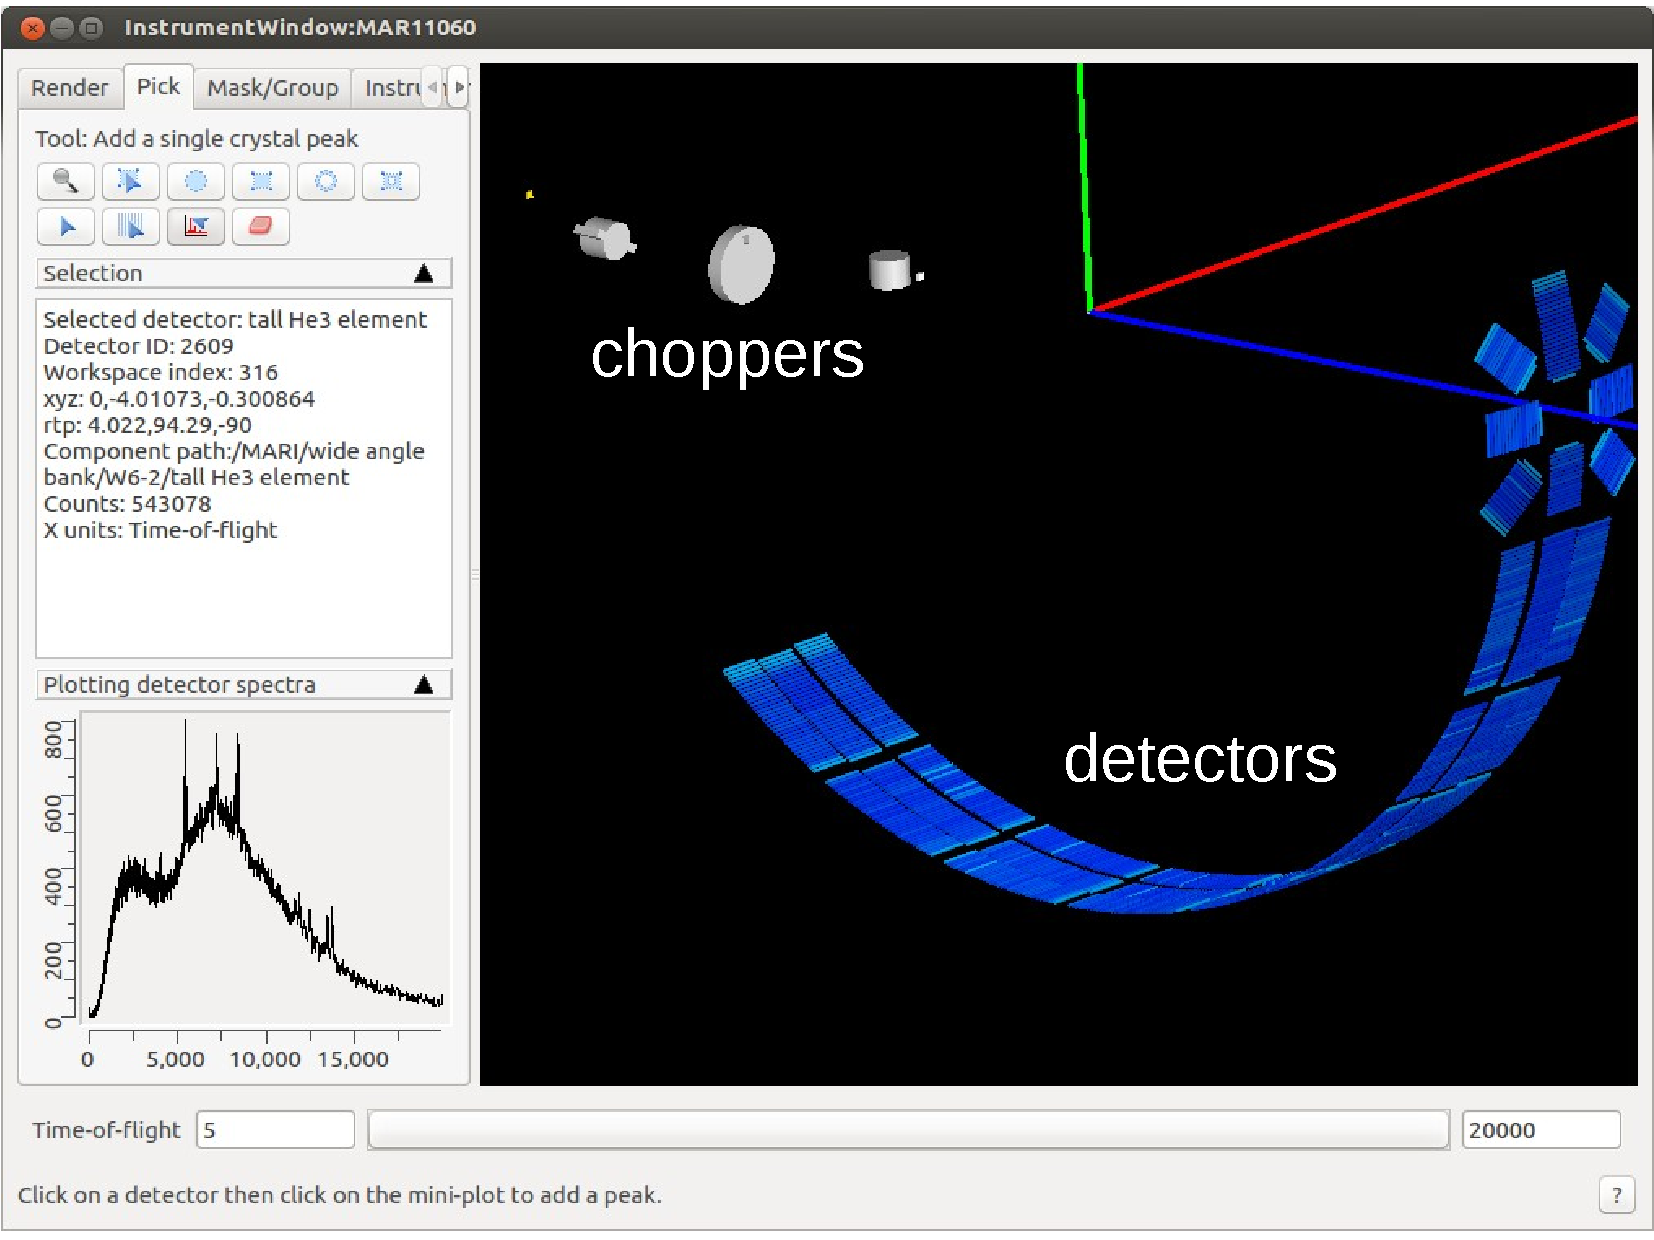
\includegraphics[width=0.75\textwidth]{instrumentview.pdf}}
\caption{The instrument view GUI in MantidPlot showing a 3D representation of the MARI spectrometer. Various components are annotated.  }
\label{fig:InstrumentView}
\end{figure}

\subsection{Slice viewer}

One tool for visualising multi-dimensional (MD) data is the SliceViewer (Figure \ref{fig:SliceView}). The SliceViewer provides an interactive 2D projection of multiple data types, both common 2D data and MDWorkspaces
Advanced features provide interactive line integration or overplotting integrated or non-integrated single crystal peak locations and regions. 


\begin{figure}[!htb]
\centerline{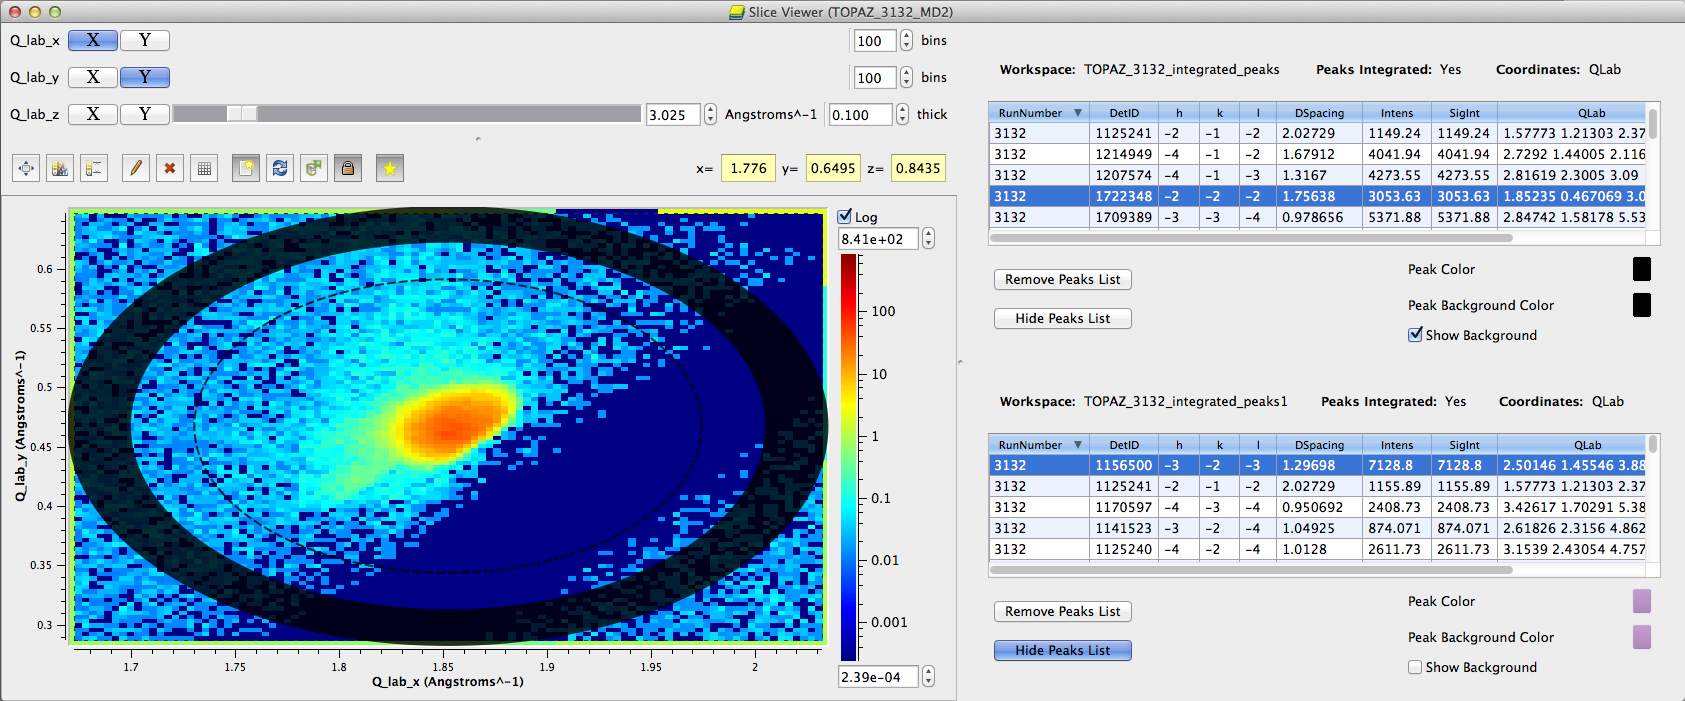
\includegraphics[width=0.75\textwidth]{Peaks_view.png}}
\caption{SliceViewer showing a single crystal peak and related information.}
\label{fig:SliceView}
\end{figure}


\subsection{VATES}\label{VATES}
A major objective of this project has been the ability to represent multidimensional data \cite{DAVE, Mslice, Horace}. Originally the Visualization and Analysis Toolkit Extensions (VATES) project was an add-on to Mantid that is now fully integrated into the project. For visualising 3 or more dimension datasets, Mantid provides several options. 


\begin{figure}[!ht]
\centerline{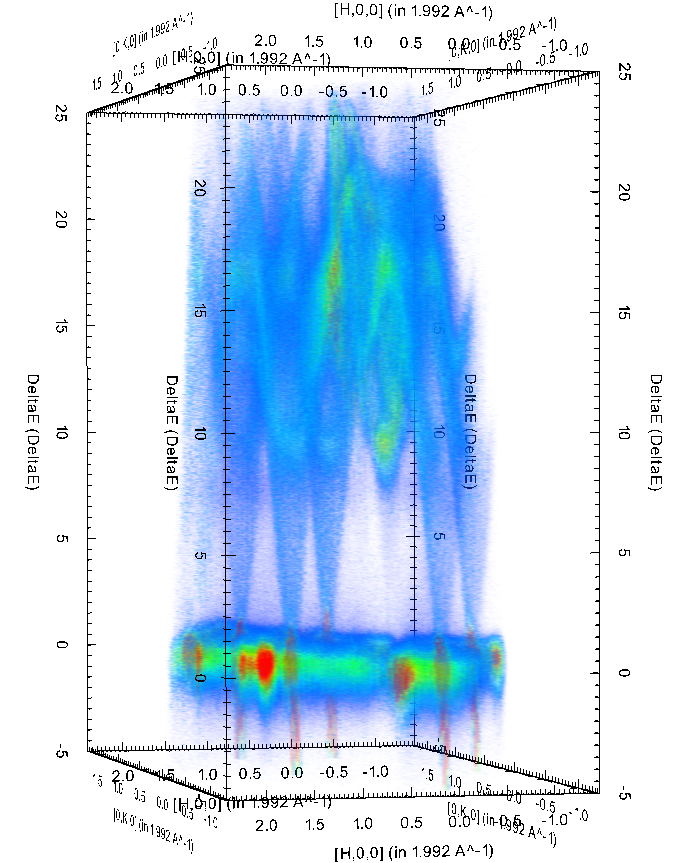
\includegraphics[width=0.6\textwidth]{NonOrthogonalProjection_W.png}}
\caption{Volume rendering of Gd excitations, in ParaView. Data was measured on SEQUOIA spectrometer at SNS.}
\label{fig:ParaView_sample}
\end{figure}


\begin{figure}[ht]
\centerline{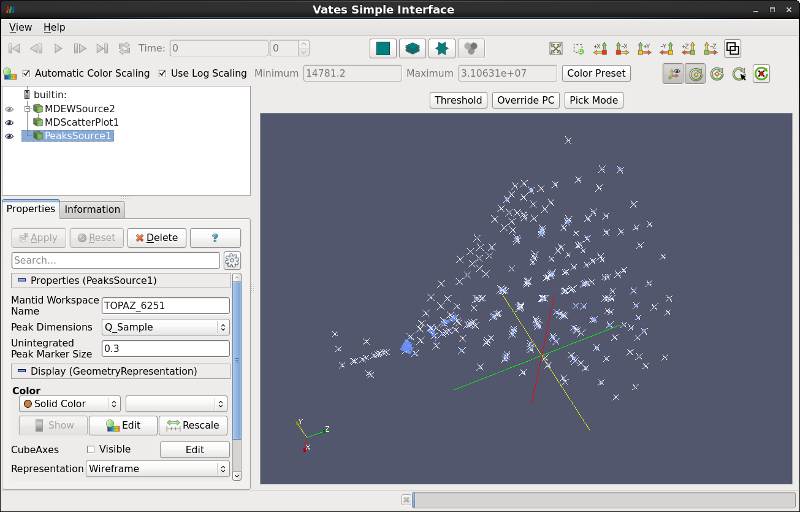
\includegraphics[width=0.75\textwidth]{VSI-v2-SplatterPlot.png}}
\caption{VSI in splatter plot mode with single crystal data from TOPAZ difractometer.}
\label{fig:VSI_sample}
\end{figure}

The VATES Simple Interface (\textit{VSI}), offers a stock set of data views and access to a subset of Mantid algorithms. It is based on application widgets and rendering libraries from the ParaView\cite{paraview} visualization program. The \textit{VSI}$\*$ takes advantage of the ParaView plugin architecture to provide functionality from within Mantid and from within ParaView standalone. The data in Mantid to be visualised passes through an API layer which translates the internal Mantid data structure to a VTK\cite{vtk} data structure, that can be rendered in the \textit{VSI}$\*$. Those same data structures can be saved to file and visualised in the ParaView program. Indeed, it is possible to drive some aspects of multidimensional analysis directly from ParaView. The API layer provides the desired decoupling of the data structures and provides good flexibility to handle the various needs of the Mantid data structures and algorithms. 



The \textit{VSI} has a view called MultiSlice which allows placing multiple orthogonal slices on the data. Those slices can then alternately be viewed in SliceViewer. The SplatterPlot (Figure \ref{fig:VSI_sample}) view is oriented towards visualising peaks in single crystal diffraction data. In that view the user can interact with the data to retrieve information about a selected peak. The ThreeSlice view shows three orthogonal planes through the data with the capability exploring via moving a crosshair in one of the planes with a coordinate readout in each plane to show the location. The \textit{VSI}$\*$ has the ability to show the data with non-orthogonal axes such as the data in Figure \ref{fig:ParaView_sample}. This capability was implemented by Kitware\cite{kitware} via the SNS in support of the Mantid project.

Ongoing work on the VATES interface aims to provide full scriptable control over all the visualization tools described, as well as increased support for multidimensional processing in technique specific areas. 


\section{Community involvement and expandability}
The Mantid framework provides facility users with a very powerful data analysis tool. The python API gives the user the ability to expand functionality for many different applications. User generated python applications can be submitted to the Mantid script repository. The script repository  allows users to contribute and share scripts with the rest of the Mantid community and MantidPlot allows upload and downloading as well as marking scripts to automatically updated with new versions from the  repository. The flexible nature of the framework can be used to analyse most types of experimental data, and is often used in new and interesting ways by the community that were not originally envisaged by the development team.
With the many algorithms supported by Mantid extensive documentation is required,  This is provided at several levels, from helpful validation,"intellisense" style help within the scripting environment, offline help provided with the installation and online help including examples and tutorials.
Finally the MantidPlot application allows users to submit bug reports, requests for assistance or just a suggestions for future development directly to the development team.

\section{Facility integration}
A very important step in Mantid development and deployment is facility integration with systems for locating files within the facilities data archive and accessing the metadata catalog for experiments.  To assist in this Mantid interfaces with Information CATalog (ICAT) \cite{ICAT}, and each facilities data archive through a plug in interface. 

The ICAT cataloguing software provides a well defined API to interface with data at large research facilities. It is in use at both ISIS and SNS, and provides a mechanism to link all aspects of the research chain, from proposal through publication. Each facility uses a different approach to storing their archived data files, Mantid allows a small archive search adapter to be written to a provided interface to locate raw or processed files in data archives at each of the facilities.
One important use of the ICAT interface and Mantid is the autoreduction process in use on certain instruments. As soon as files are created and catalogued, a reduction script is automatically invoked. This script uses metadata in the file and/or the ICAT catalogue to reduce the raw file to a format that contains the data that users are interested in. 

In addition at SNS and ISIS, the development team has developed the interface between Mantid and the data acquisition systems, in order to allow users to look and analyse their data in real time, before a file is even written to the disk.   This approach captures either events as they stream off the data acquisition or point in time histograms, and allows for near real time processing of the results into scientifically useful results. This level of near real time data analysis allows for much better planning and use of valuable experiment time.  


\section{Conclusion}
The Mantid project offers an extensible framework for data manipulation, analysis and visualization, geared toward neutron scattering and $\mu SR$ experiments. It is the main reduction software in use at SNS and ISIS, and partially in use or considered at several other scientific facilities. Up to date information, and usage tutorials can be found on the Mantid web page\cite{webpage}. 

\section{Acknowledgements}
The development team would like to thank all instrument scientists and ISIS and SNS for their feedback and help. Work at ORNL was sponsored by the Scientific User Facilities Division, Office of Basic Energy Sciences, US Department of Energy. Work at the ISIS facility was funded by the Science and Technology Facilities Council (STFC) UK. Development for ILL instruments was funded by NMI3 (WP6)

\begin{center}
\line(1,0){250}
\end{center}
% The Appendices part is started with the command \appendix;
% appendix sections are then done as normal sections
% \appendix

% \section{}
% \label{}

\bibliography{Mantid}{}
\bibliographystyle{elsarticle-num}
\end{document}


